\begin{frame}
  \frametitle{Motivazioni}
  \begin{columns}[t]
    \begin{column}{4cm}
       \begin{block}{Deterioramento delle immagini}
         Processi di acquisizione di immagini traminte scanner 3D o di
         trasferimento delle stesse, possono deteriorale generando del
         \alert{rumore}. 
       \end{block}
     \end{column}
     \begin{column}[T]{6cm}
      \only<2>{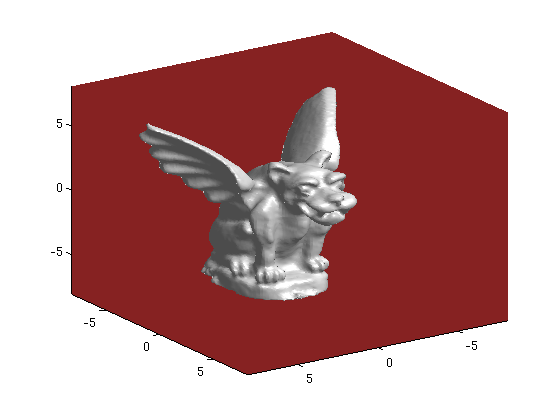
\includegraphics[width=1.0\textwidth]{smooth/mcm/gargolye/garg149-0-00}}
      \only<1>{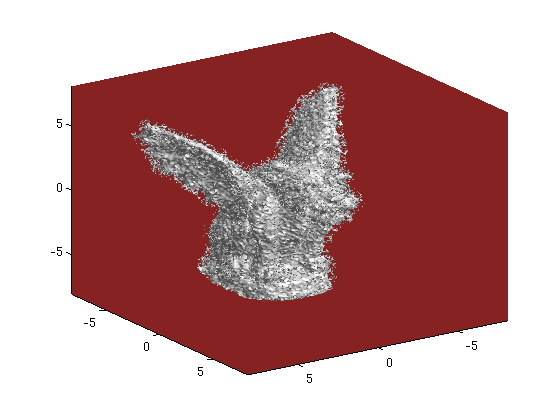
\includegraphics[width=1.0\textwidth]{noise/imnoise/mcm/gargolye/garg149i-0-00}}
      \only<3>{
        \begin{block}{PDE per il filtraggio}
          \begin{itemize}
            \item Concetto di \emph{multi-scala}, l'immagine iniziale
              viene racchiusa in una famiglia dipendente dalla scala $t$
            \item \emph{Multi-scala} ottenuto come soluzioni di PDE
              evolutivi
            \item Equazione del calore
            \item Moto per curvatura media
            \item \alert{Moto per curvatuta media che preserva il volume}
          \end{itemize}
          \end{block}}
     \end{column}
  \end{columns}
\end{frame}
